\subsection{摘要：打破三堵墙}

本节讨论了教育部高效培训的三个基本障碍，每一个障碍都是硬性约束，如果不解决，就会阻碍大规模的实际培训。

\begin{itemize}
    \item \textbf{记忆墙}：内存是第一个限制。如果参数、优化器状态和激活超出 GPU 容量，则训练无法继续。内存高效排列、FP8/FP4 激活、细粒度重新计算、卸载、精度感知优化器和 FSDP 一起将 DeepSeek-V3 的 199.5 GB 每 GPU 要求转换为可行的训练配置。

    \item \textbf{通讯墙}：通信开销直接降低了GPU利用率。优化调度程序（DeepEP、HybridEP）最大化带宽，FWD-BWD 重叠隐藏计算背后的延迟。总之，这些措施可将整体开销从多达 60\% 训练时间少于10\% 在 DeepSeek-V3 训练中。

    \item \textbf{计算效率墙}：计算效率低下有两个原因：未充分利用 GPU 资源的小内核，以及导致 GPU 闲置的主机开销。分组GEMM和内核融合提高内核效率； CUDA 图形和无同步 MoE 消除了主机开销。这些将计算效率低下从主要瓶颈转变为可管理的约束。
\end{itemize}

这些优化不是独立的。它们形成了一个连贯的系统，其中一堵墙的解决方案可以启用或增强其他墙的解决方案。降低精度的训练清楚地表明了这一点：它减少了内存（激活）并提高了计算效率（更快的 Tensor Core 操作），同时需要仔细集成以避免引入新的瓶颈（量化内核开销）。

以下各节解决了两个交叉问题：第~\ref{sec:reduced-precision-training} 涵盖 FP8/FP4 中的降低精度训练，同时影响所有三堵墙，以及部分~\ref{sec:long-context-training} 解决长上下文 MoE 训练问题，当注意力主导计算时，这会改变优化平衡。


%==============================================================================
% SECTION 5: Low PRECISION TRAINING - THE FP8 JOURNEY
%==============================================================================

\section{教育部 FP8/FP4 的降精度训练}\label{sec:reduced-precision-training}

前面的部分针对三堵墙进行了针对性的优化。降低精度训练是独一无二的：它同时影响内存、通信和计算效率，使其成为值得专门处理的跨领域优化。

混合精度训练一直是高效深度学习的基石，以 BF16 为标准实践 \cite{micikevicius2018mixed,peng2023fp8lmtrainingfp8large,xi2024coat}。 FP8/FP4 中的降低精度训练代表了更激进的一步，将精度从 16 位降低到 8 位甚至 4 位，相应的收益和风险也更大 \cite{micikevicius2022fp8formatsdeeplearning,fishman2025scalingfp8trainingtrilliontoken}。对于 DeepSeek-V3，FP8 训练将每个 GPU 的激活内存减少了大约 16 GB，通过更快的 Tensor Core 操作改进了专家 GEMM，并加速了参数 AllGather 通信。这些收益在三堵墙之间复合，使得 FP8 对于高效的大规模 MoE 培训至关重要。

然而，低精度训练会带来收敛风险，必须系统地解决。本节介绍 Megatron-Core 的降低精度训练方法：了解精度的重要性，选择适当的量化方案，以及实施 MoE 特定的优化，以获取降低精度训练的优势，同时保持训练稳定性。

\subsection{为什么低精度训练对教育部很重要}\label{sec:precision-anatomy}

与密集模型相比，MoE 架构放大了低精度训练的好处和风险：

\textbf{扩大效益。} 有了数百名专家，激活记忆就会成比例地扩展。 FP8/FP4 激活比密集模型提供更大的绝对内存节省。参数 AllGather 的通信量减半\footnote{对于 Blackwell 上的 NVFP4 配方，由于我们需要收集行向和列向权重张量，因此节省的通信量也是 50\%.}，而专家 GEMM（主导 MoE 计算）受益于更快的 Tensor Core 吞吐量。

\textbf{风险放大。} 路由器决策取决于精确的分数来将令牌分配给专家。量化噪声可能会破坏专家选择的稳定性，导致训练不稳定、模型质量下降或专家崩溃 \cite{nagel2021whitepaper}。必须保护数字敏感组件免受过度量化。

\textbf{策略：选择性精准。} 解决方案在重要的地方是精确的，在其他地方是效率的。指导教育部部署降低精度训练的三个原则：
\begin{enumerate}
    \item \textbf{保护路由决策。} 路由器仍为FP32，以确保稳定的专家选择。
    \item \textbf{保持关键部件的精度。} 嵌入、输出层、主梯度、主权重和优化器状态保持原始精度以保持模型质量。
    \item \textbf{量化批量计算。} 专家 GEMM 构成了大部分计算，使用经过精心设计的量化方案（称为 \textit{食谱}).
\end{enumerate}

\begin{notebox}
成功降低精度的 MoE 训练的关键是选择性精度：将数值敏感组件（路由器、嵌入、输出层、梯度和优化器状态）保持在更高的精度，同时积极量化大量计算（专家 GEMM）。该策略获得了降低精度训练的大部分好处，同时避免了收敛问题。
\end{notebox}

\subsection{降低精度训练对所有三堵墙的影响}

降低精度训练为所有三个性能墙提供了优势，使其成为统一的优化。表~\ref{tab:fp8-impact-summary} 总结了这些影响。

\begin{table}[ht]
\centering
\begin{threeparttable}
\caption{降低精度训练对三堵墙的影响摘要。}
\label{tab:fp8-impact-summary}
\begin{tabular}{lll}
\toprule
\textbf{墙} & \textbf{降低精度训练的好处} & \textbf{细节} \\
\midrule
记忆 & 50\% (FP8)/75\% (FP4) 活化减少 & 部分~\ref{sec:fp8-activation} \\
        & 消除BF16重量副本 & 部分~\ref{subsec:fp8-primary-weights} \\
        & BF16 优化器状态 & 部分~\ref{sec:precision-opt} \\
\midrule
沟通 & 50\% 参数全部收集 \tnote{1} & 部分~\ref{subsec:fp8-primary-weights} \\
\midrule
计算 & 更快的张量核心 GEMM & 部分~\ref{sec:fp8-training} \\
        & 量化内核开销 & 部分~\ref{sec:kernel-fusion} \\
\bottomrule
\end{tabular}
\begin{tablenotes}
    \footnotesize
    \item[1] 对于NVFP4，我们需要同时收集行方向和列方向的FP4权重，因此参数AllGather减少的流量也是50\%.
\end{tablenotes}
\end{threeparttable}
\end{table}

\subsubsection{通过降低精度的训练打破记忆墙}

降低精度训练通过三种方式减少内存消耗：

\textbf{激活记忆（详见章节~\ref{sec:fp8-activation}).} 激活内存节省的主要来源来自为向后计算而保存的线性层的输入张量。通过将这些张量存储在 FP8/FP4 而不是 BF16 中，内存占用量减少了 50\%/75\%。例如，FP8 为 DeepSeek-V3 的每个 GPU 节省了大约 16 GB 的激活内存。

\textbf{参数记忆。} 传统的降低精度训练维护三个参数副本：FP32 主权重、BF16 模型权重和 FP8/FP4 计算权重。我们的 \emph{原生 FP8/FP4} 方法（详见第~\ref{subsec:fp8-primary-weights} 下面）通过将权重直接从 FP32 铸造到 FP8/FP4 并以降低的精度执行参数 AllGather 来消除 BF16 副本。

\textbf{优化器状态内存（详见章节~\ref{sec:precision-opt}).} Adam 优化器状态（第一和第二时刻）可以存储在 BF16 而不是 FP32 中，从而将优化器内存减少 50\%。这与降低精度的训练正交，也适用于 BF16。

\subsubsection{通过降低精度的训练打破沟通障碍}
\label{sec:comm_wall_quantized_training}

% \textbf{FP8 EP Dispatch (detailed in Section~\ref{sec:fp8-dispatch-comm}).} For fine-grained MoE models with large EP sizes, all-to-all communication becomes a primary bottleneck. By dispatching tokens in FP8 instead of BF16, the communication volume is halved. The key challenge is managing the dequantization-quantization cycle required because forward and backward passes use different quantization dimensions.

\textbf{FP8/FP4 中的参数 AllGather。} 当使用带有分布式优化器的 FP8/FP4 主权重时，参数 AllGather 通信减少 50\% （每个参数 1 个字节与 2 个字节）。注意
\begin{itemize}
    \item 对于NVFP4，我们需要同时收集行方向和列方向的FP4权重，因此参数AllGather减少的流量也是50\%.
    \item 对于 MXFP8，即使使用 FP8 主权重，我们也首先将 FP32 主权重复制到临时 BF16 缓冲区中，并以 BF16 精度进行通信。这是因为 MXFP8 需要向前和向后传递不同的量化方向。通信 MXFP8 权重需要行式和列式量化版本，每个参数有效地通信两个字节，并且消除了与 BF16 通信相比的任何优势。因此，对于 MXFP8，我们以 BF16 精度传递参数。 
\end{itemize}

\subsubsection{通过降低精度的训练打破计算效率壁垒}

\textbf{更快的 GEMM。} FP8（Ada/Hopper 及更高版本）和 FP4（Blackwell 及更高版本）Tensor Core 提供比 BF16 更高的吞吐量，加速前向和后向传递。

\textbf{权衡：量化开销。} 降低精度的训练引入了额外的量化内核，从而增加了 CPU 开销，这对于细粒度 MoE 来说尤其成问题，因为许多小操作已经给 CPU 带来了压力。该开销通过以下方式管理：
\begin{itemize}
    \item \textbf{内核融合} 将量化与其他操作融合在一起，例如标准化和激活函数。
    \item \textbf{熔丝填充/取消填充} 使用排列内核或路由映射来避免显式填充/取消填充。
    \item \textbf{分组量化} 它将多个输入张量的量化融合到一个内核中。
    \item \textbf{CUDA 图形} 捕获量化内核以消除启动开销。见章节~\ref{sec:cuda-graphs} 了解更多详情。
\end{itemize}

\subsection{降低精度训练方案：每张量 FP8、Blockwise FP8、MXFP8 和 NVFP4}

在确定了降低精度训练对所有三面墙的影响后，我们现在检查定义降低精度训练配置的技术组件。

\begin{figure}[ht]
    \centering
    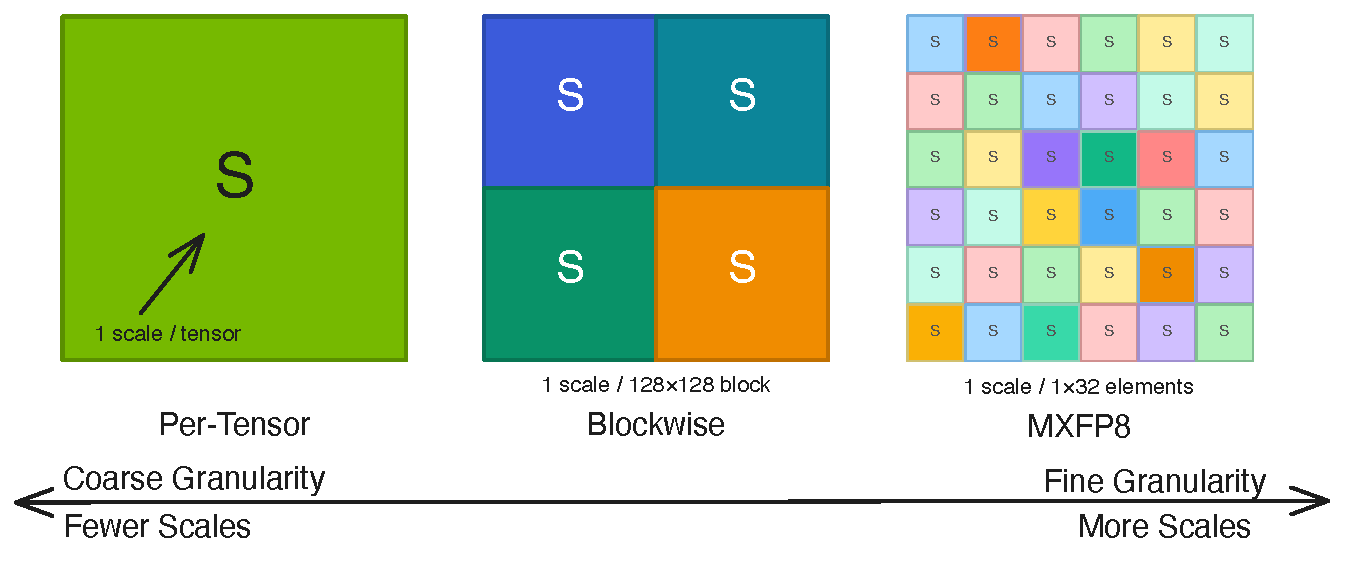
\includegraphics[width=0.9\textwidth]{figures/plots/fp8_recipes_comparison_draft.pdf}
    \caption{FP8 训练方法：每张量缩放、Blockwise FP8 和 MXFP8。}
    \label{fig:fp8-recipes-overview}
\end{figure}

降低精度的训练方法包括：
\begin{itemize}
    \item \textbf{数据格式。} FP8格式有两种：E4M3和E5M2 \cite{micikevicius2022fp8formatsdeeplearning,kuzmin2022fp8quantization}。通常在训练中使用两种组合：
    \begin{itemize}
        \item \textbf{E4M3}：输入、权重和梯度均以 E4M3 格式量化。
        \item \textbf{杂交种}：输入和权重在 E4M3 中量化，而梯度在 E5M2 中量化。
    \end{itemize}
    而对于 FP4，E2M1 是唯一支持的格式。
    \item \textbf{缩放粒度。} 选项包括每个张量和每个块（也称为组或图块）。对于每块缩放，块大小也因配方而异。
    \item \textbf{哪些部分被量化。} 通常所有线性层都会被量化，同时保持嵌入、输出层（LM头）和优化器的原始高精度。部分通信可以采用 FP8/FP4（例如 TP AllGather、DP AllGather、EP all-to-all）。当前降低精度的训练方案通常将 SDPA 保留在 BF16 中。
    \item \textbf{附加机制}，例如随机舍入、随机 Hadamard 变换 (RHT) 等。这些机制是特定于配方的，需要仔细验证。 
\end{itemize}

Megatron-Core 提供了三种 FP8 配方，每种配方均经过大规模验证（\figref{fig:fp8-recipes-overview}）。从按张量到按块再到 MXFP8 的演变反映了硬件进步和大规模部署的经验教训。 \textbf{每张量缩放} 每个张量使用单个比例因子，简单但精度有限，适合实验。 \textbf{块式 FP8} (128$\times$128 个块）提供更细的粒度，并具有经过验证的规模稳定性，推荐用于 Hopper。 \textbf{MXFP8} (1$\times$32 粒度）提供原生 Blackwell Tensor Core 支持和硬件加速缩放（推荐用于 Blackwell）。此外，Megatron-Core还提供了NVFP4配方 \cite{nvidia2025pretraininglargelanguagemodels} 在布莱克威尔。

\subsubsection{每张量 FP8 配方}
Hopper 和 Blackwell 支持的每张量 FP8 配方通常采用混合格式（E4M3 用于输入/权重，E5M2 用于梯度）。它计算输入张量中所有值的绝对最大值 (amax)，并使用该值将张量量化为 FP8。

每个张量缩放有两种变体：
\begin{itemize}
    \item \textbf{延迟缩放}：从历史窗口使用 amax。这打破了 amax 计算和缩放之间的数据依赖性，提供了最佳性能，但存在由于估计的 amax 而损失精度的风险。
    \item \textbf{当前（实时）缩放}：及时计算 amax，提供更好的精度。
\end{itemize}

我们不建议因精度问题而延迟缩放；电流缩放提供了更好的精度和模型收敛性。
人物～\ref{fig:fp8-cs-hopper} 还有~\ref{fig:fp8-cs-blackwell} 分别说明了 Hopper 和 Blackwell 平台上具有每张量电流缩放的线性层的计算。由于 Hopper 仅支持 TN 布局 FP8 GEMM，因此我们必须存储转置的 FP8 激活以用于向后计算。在 Transformer Engine 中，量化内核将转换和转置融合到单个内核中，以减少全局内存访问。在Blackwell平台上，所有布局的FP8 GEMM都受支持，因此我们不需要转置版本，进一步减少了内存占用。

由于其简单性以及相对较好的精度和性能，每张量缩放是迁移到 FP8 训练的良好起点。


\begin{figure*}[t!]
    \centering
    \begin{subfigure}[t]{0.45\textwidth}
        \centering
        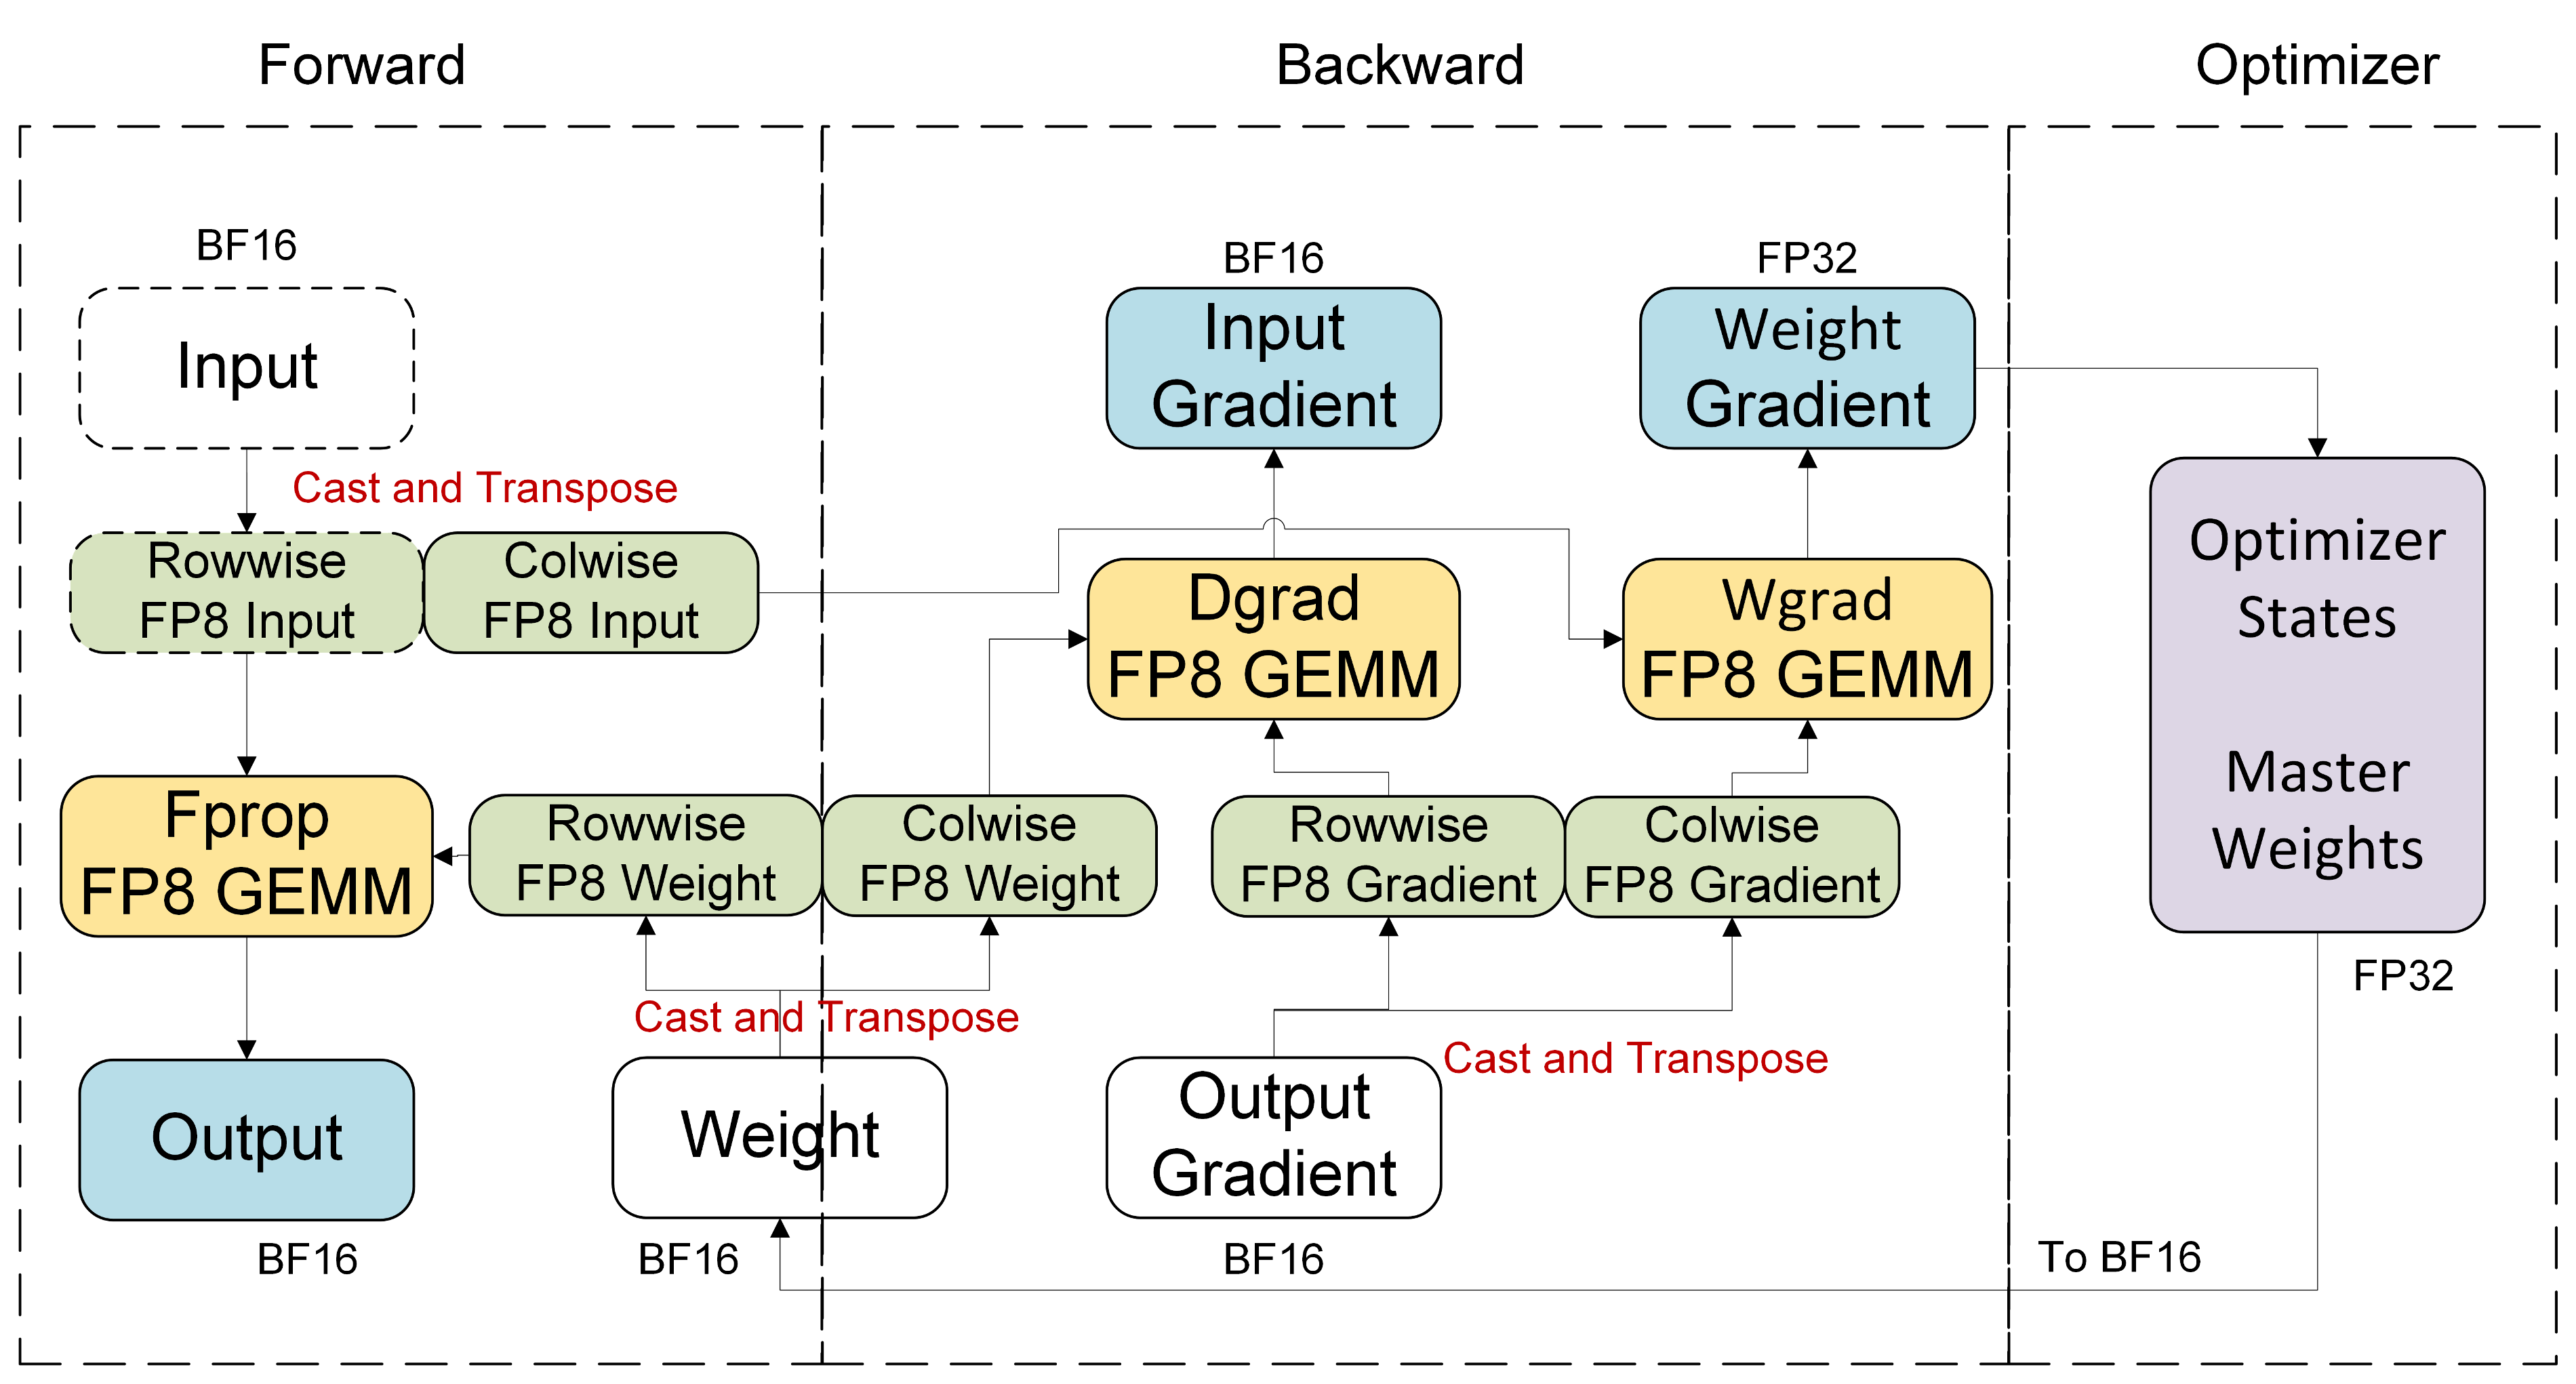
\includegraphics[width=1.0\linewidth]{figures/fp8-cs-hopper.png}
        \caption{Hopper 平台上每个张量的电流缩放。}
        \label{fig:fp8-cs-hopper}
    \end{subfigure}
    \begin{subfigure}[t]{0.45\textwidth}
        \centering
        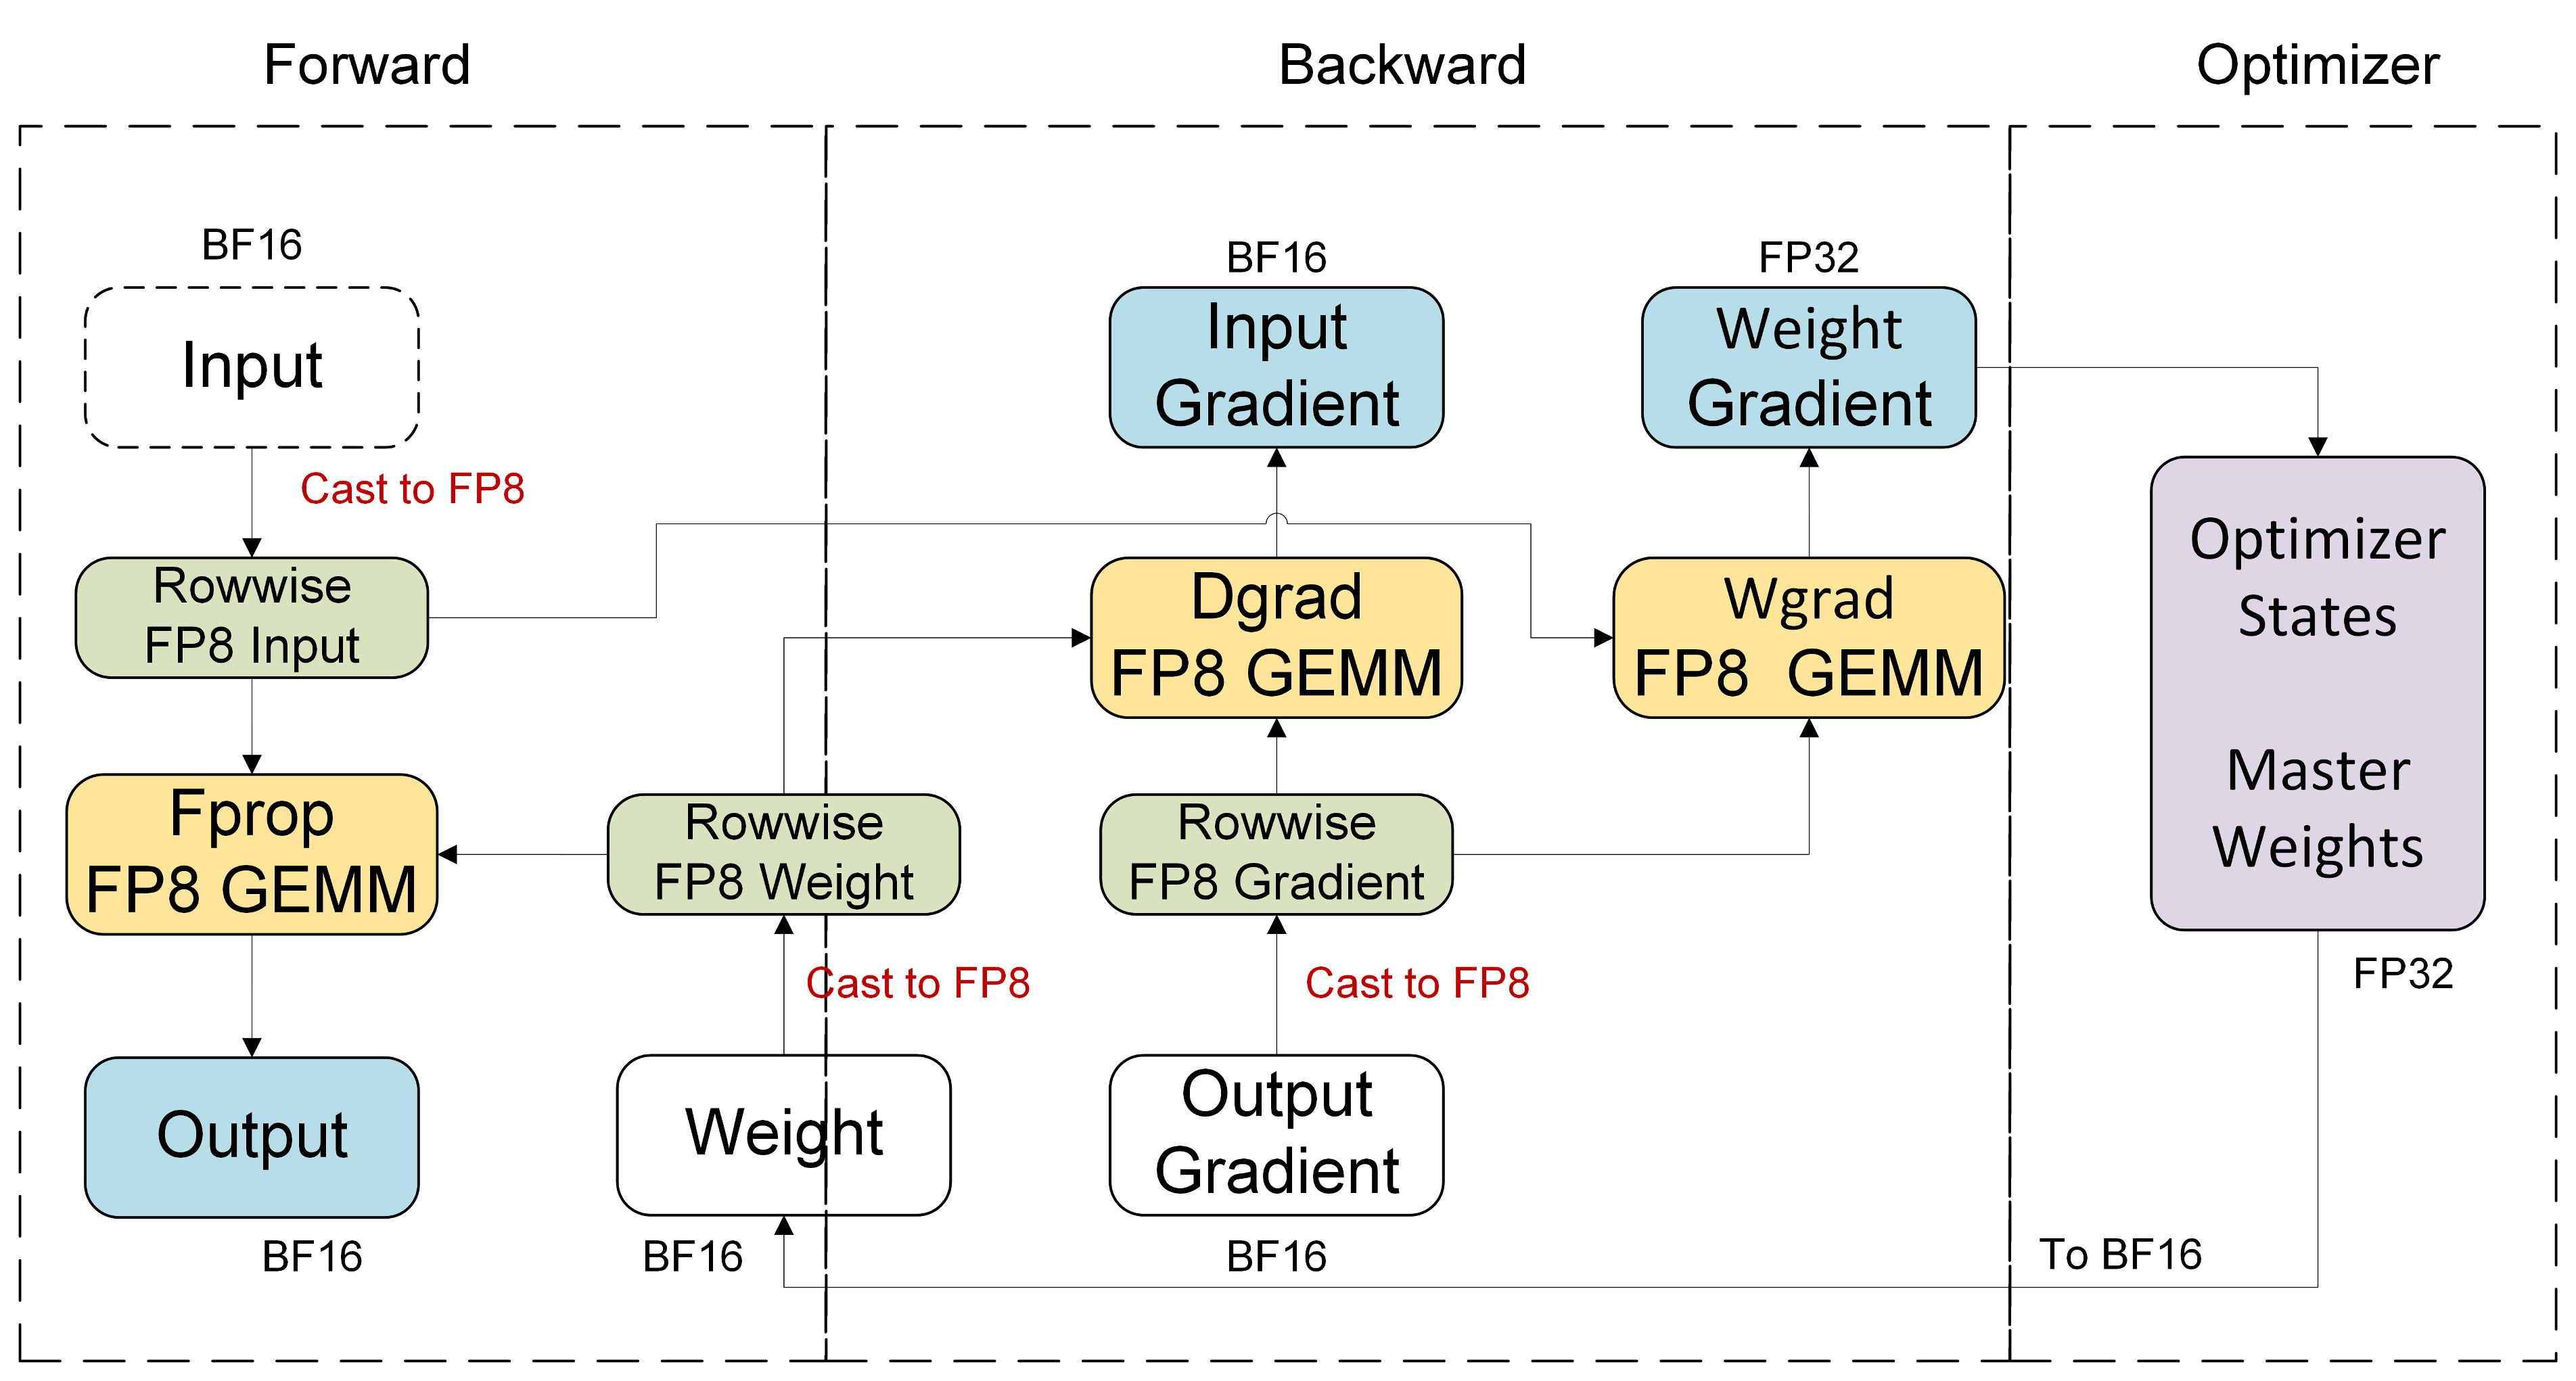
\includegraphics[width=1.0\linewidth]{figures/fp8-cs-blackwell.png}
        \caption{Blackwell 平台上的每张量电流缩放。}
        \label{fig:fp8-cs-blackwell}
    \end{subfigure}
    \begin{subfigure}[t]{0.45\textwidth}
        \centering
        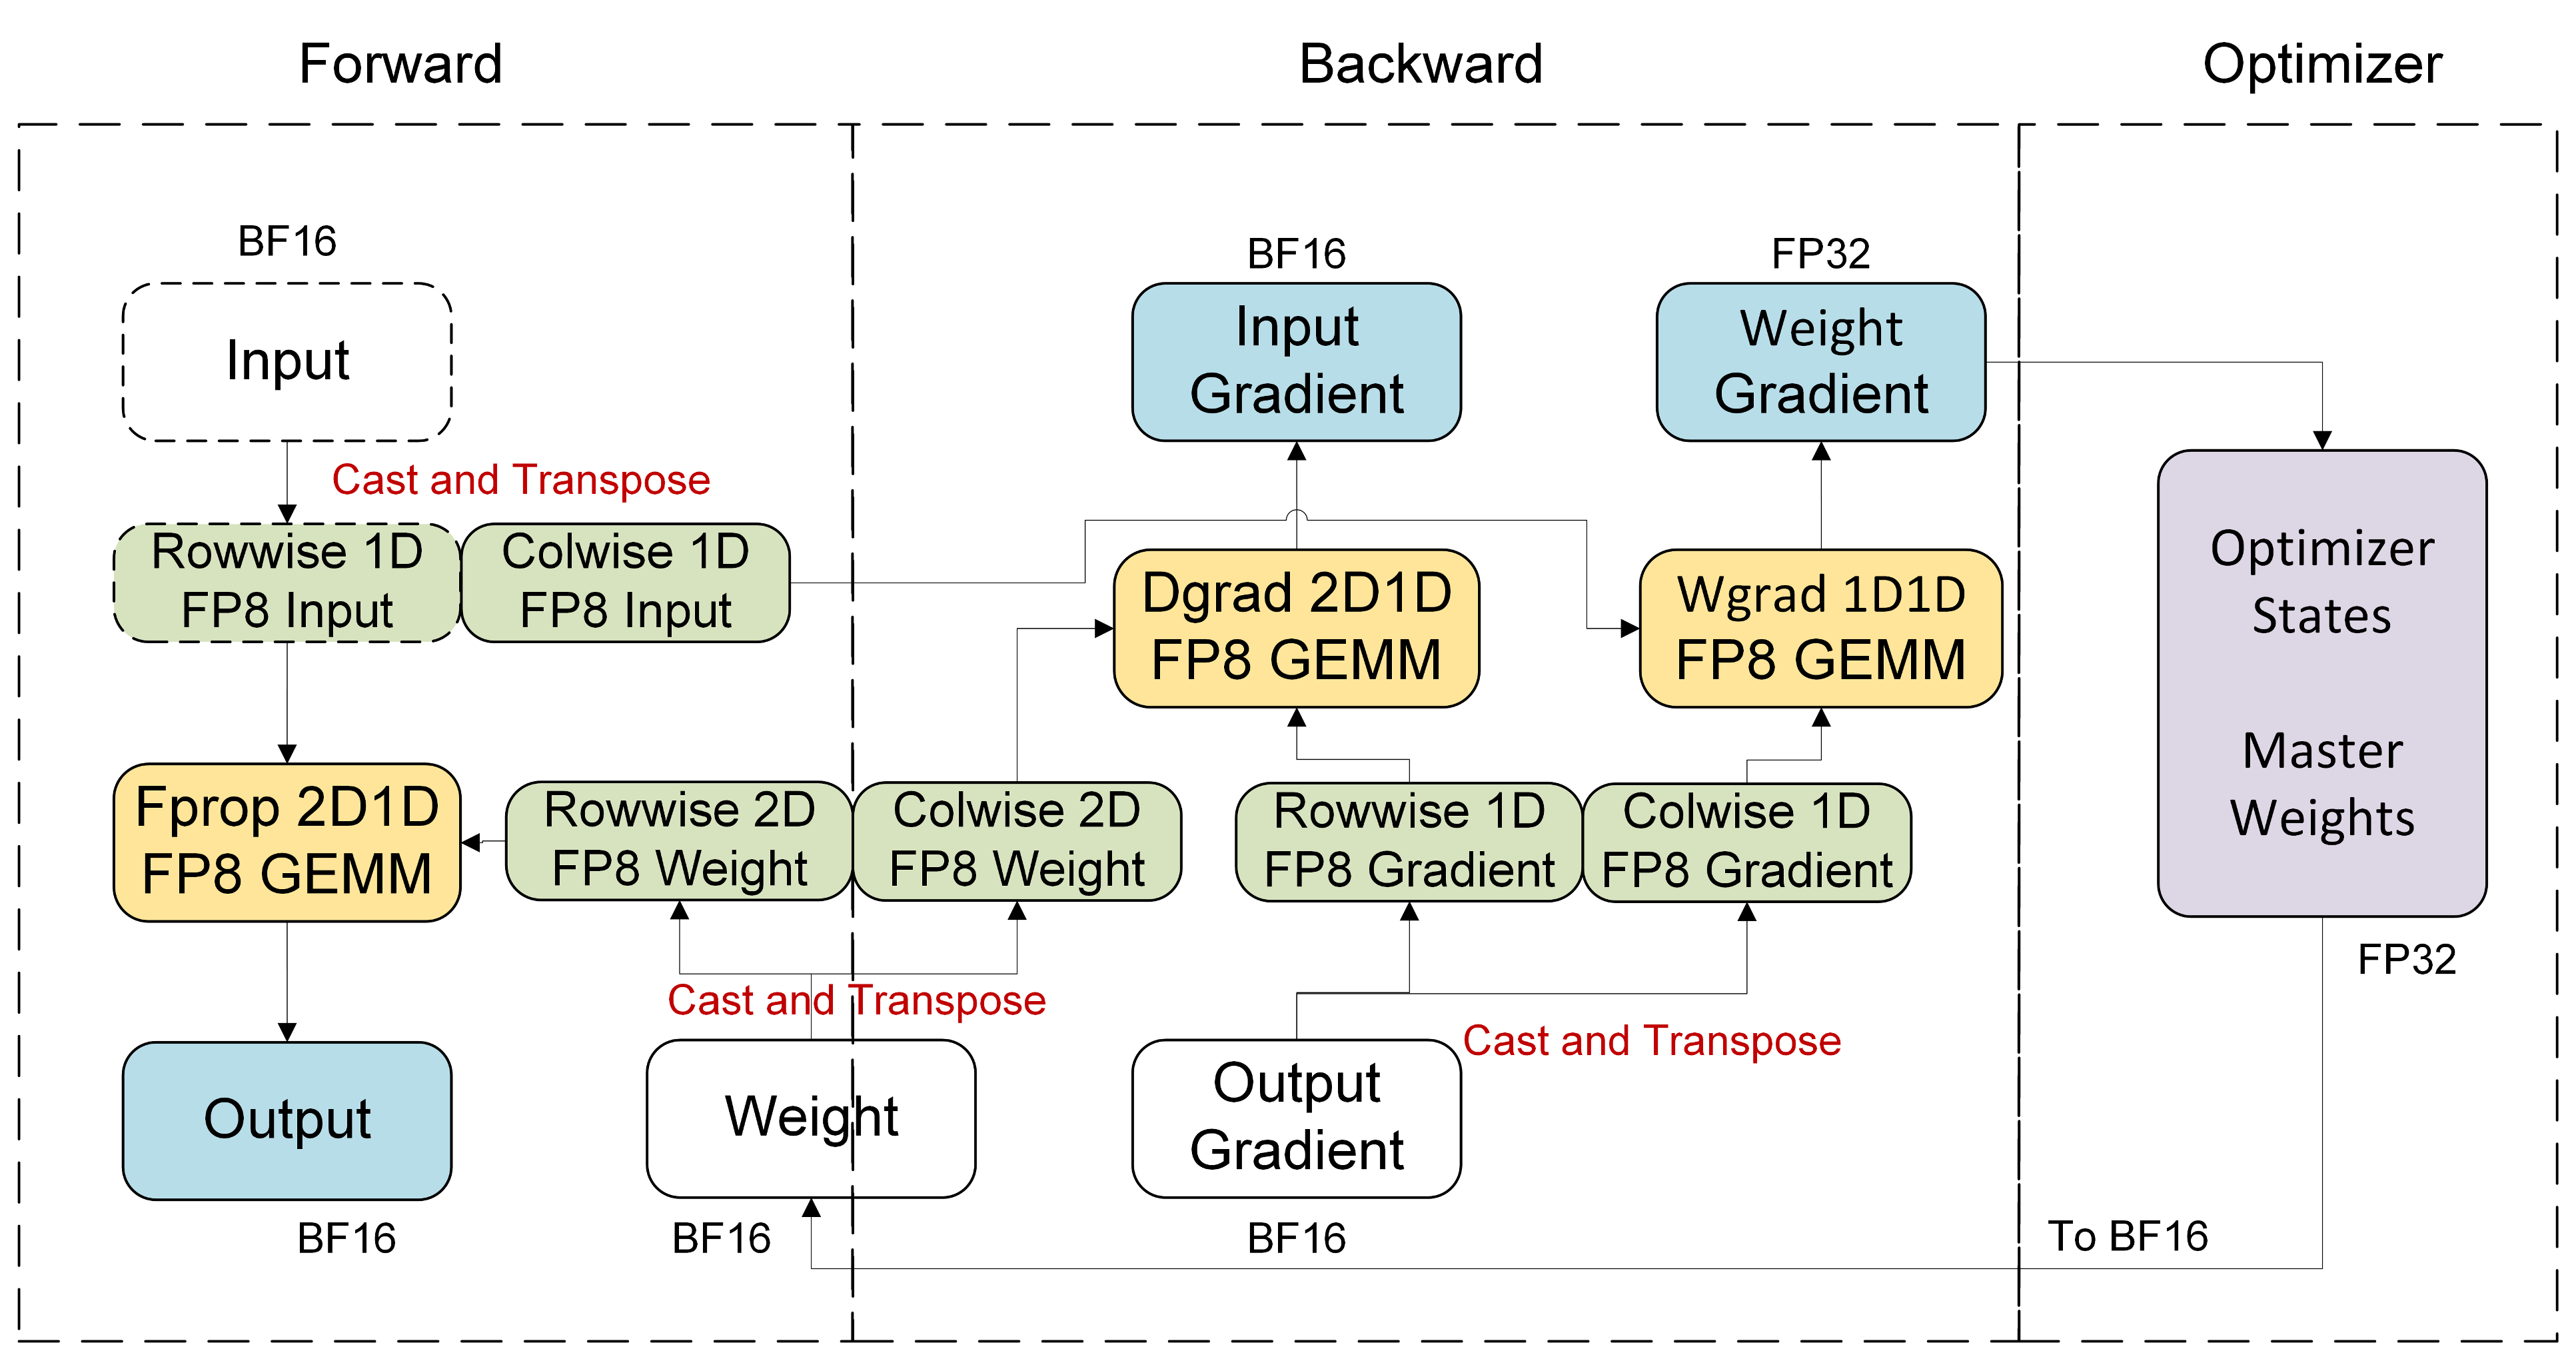
\includegraphics[width=1.0\linewidth]{figures/fp8-blockwise-hopper.png}
        \caption{Hopper 上的 Blockwise FP8 配方。}
        \label{fig:fp8-blockwise-hopper}
    \end{subfigure}
    \begin{subfigure}[t]{0.45\textwidth}
        \centering
        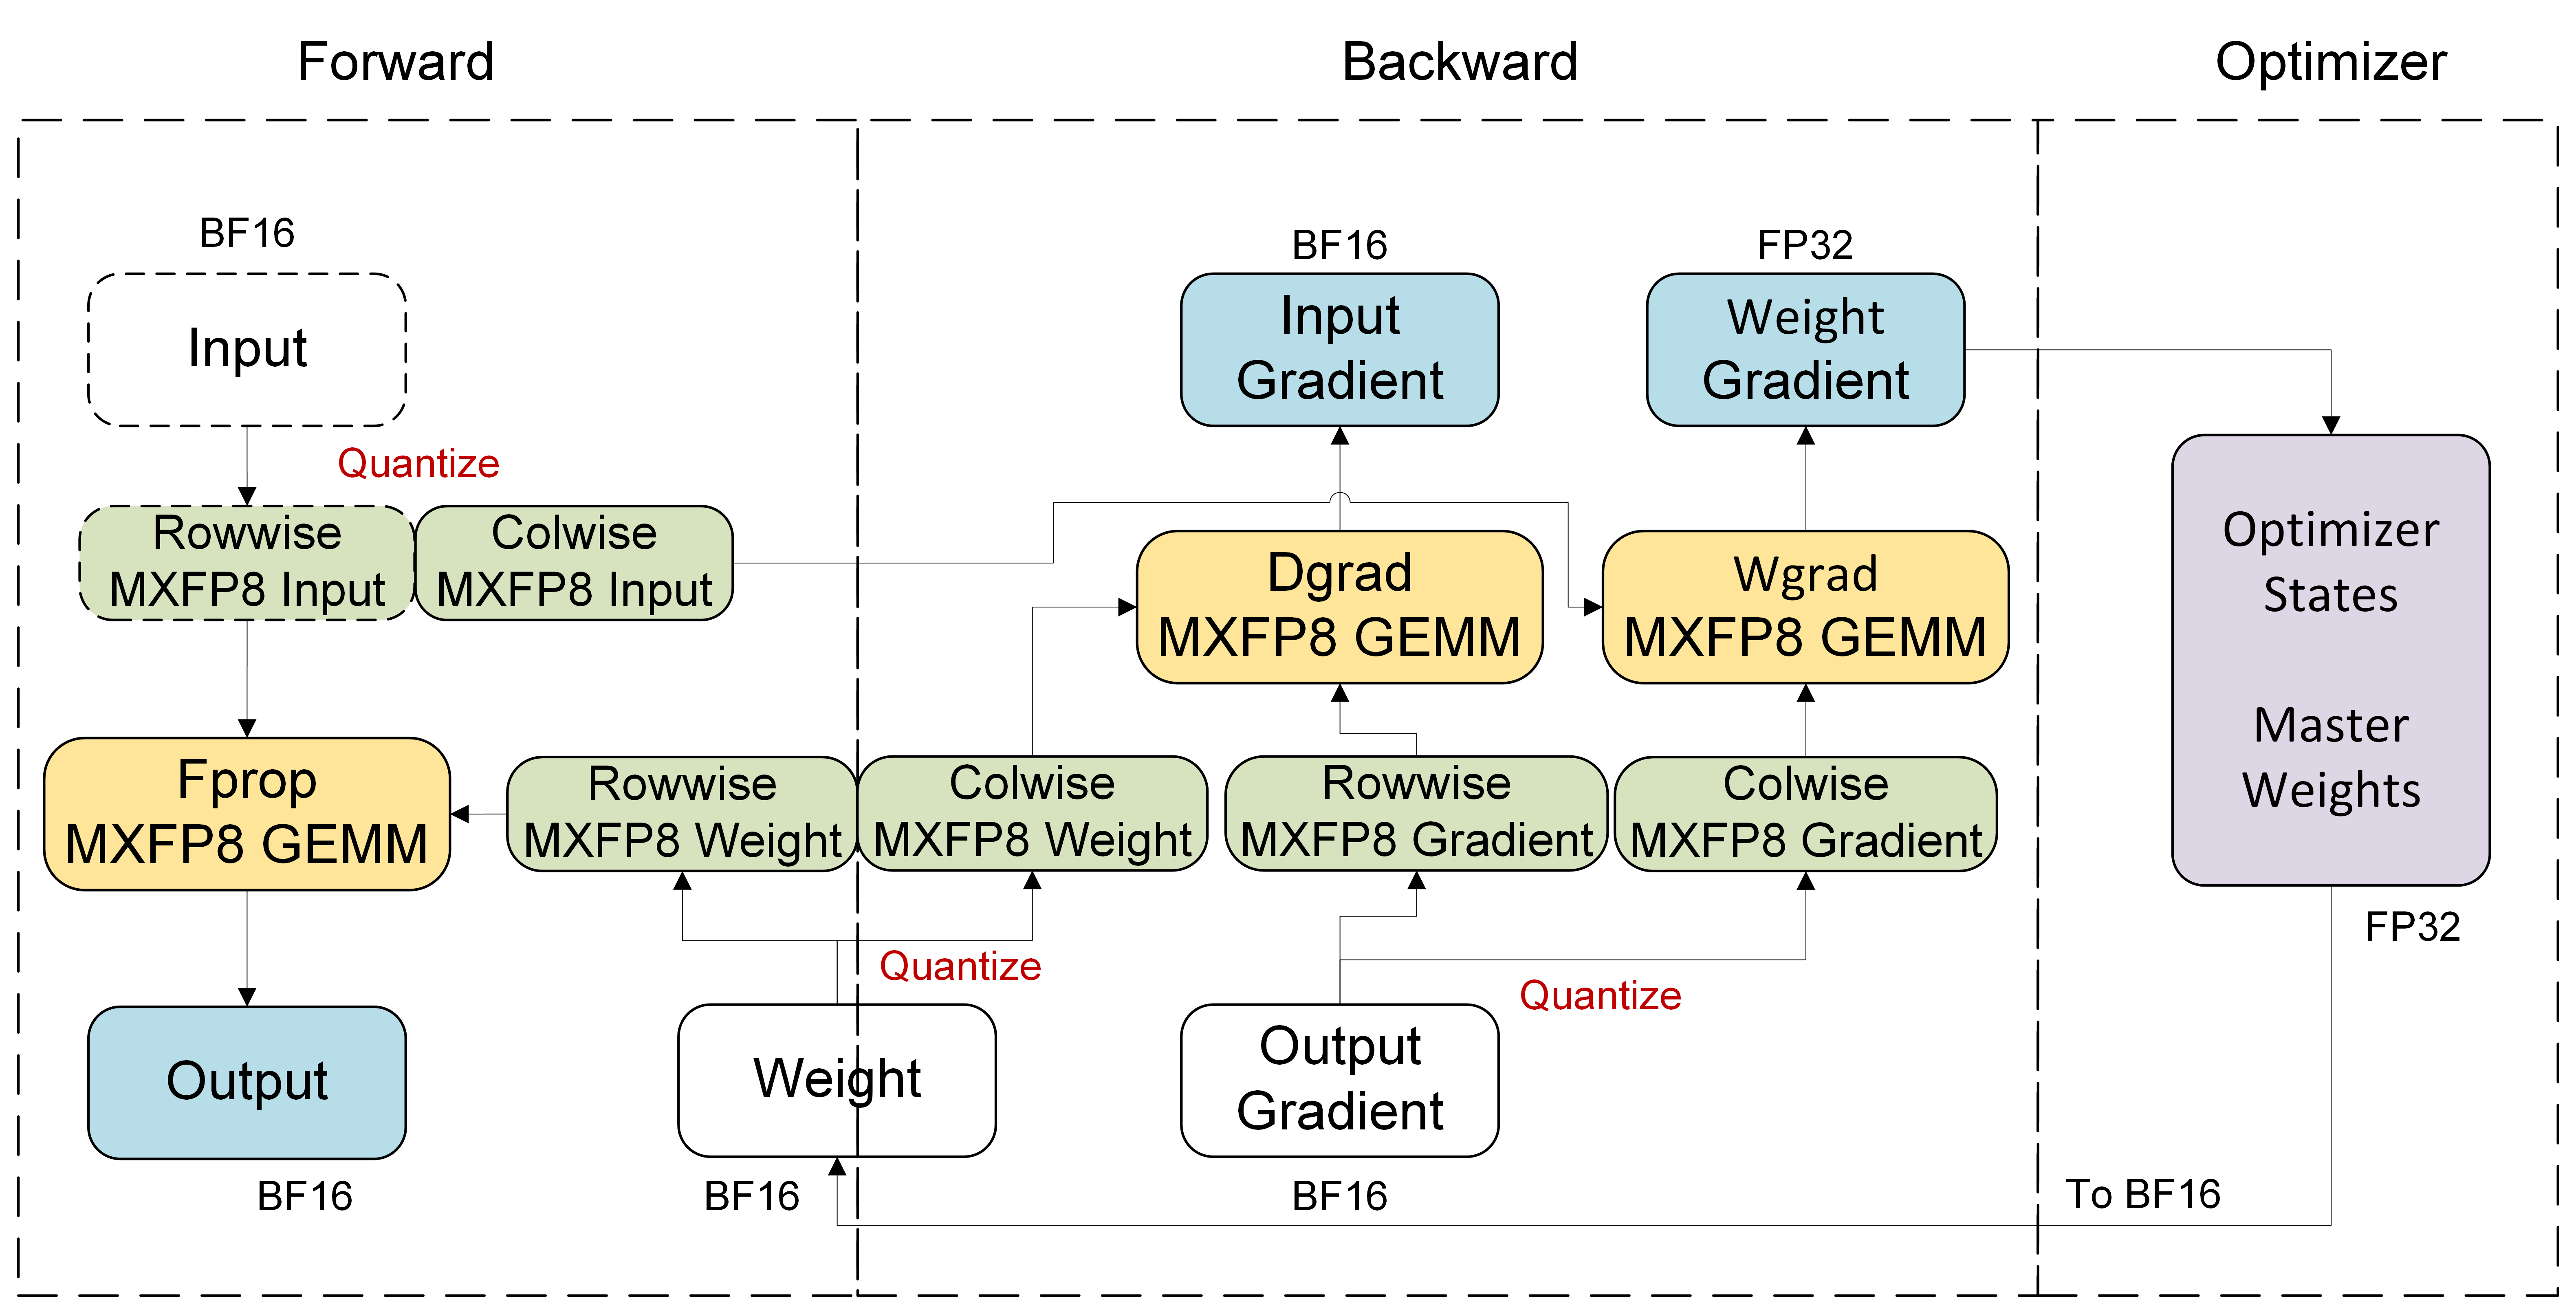
\includegraphics[width=1.0\linewidth]{figures/fp8-mxfp8.png}
        \caption{Blackwell 平台上的 MXFP8 配方。}
        \label{fig:fp8-mxfp8}
    \end{subfigure}
    \caption{使用各种 FP8 配方计算线性层。请注意跨平台量化粒度和张量布局要求的差异。}
    \label{fig:fp8-recipes}
\end{figure*}

\subsubsection{Hopper 上的 Blockwise FP8}
块式 FP8 配方对所有张量采用 E4M3 格式，量化激活和梯度 $1 \times 128$ 瓷砖和权重 $128 \times 128$ 块。块式缩放使用细粒度缩放粒度来获得更好的精度，并且已被 \textbf{已在生产中证明是成功的} 在超大规模 MoE 模型中，包括 DeepSeek-V3 \cite{deepseekai2025deepseekv3technicalreport}, 极小极大-M2 \cite{minimax_m2}、蚁灵-2.0 \cite{li2025every}等等。因此，blockwise FP8 是 Hopper 平台上推荐的 FP8 配方。

Transformer Engine 为块式配方提供高度优化的量化内核和 GEMM 内核（通过 cuBLAS），以及分层 API 和自动转换上下文，只需几行代码即可进行 FP8 训练。

\Figref{fig:fp8-blockwise-hopper} 说明了 Hopper 平台上使用分块 FP8 配方的线性层的计算，这与 Hopper 上的每张量当前缩放非常相似，除了基于图块的量化之外。

\subsubsection{布莱克威尔上的 MXFP8}
在 Blackwell 平台上，得益于原生第五代 Tensor Core 对 MXFP8 格式的支持 \cite{rouhani2023microscalingdataformatsdeep}，我们采用更细粒度的量化方案MXFP8进行训练。激活和权重都被量化为 $1 \times 32$ 粒度，E8M0用于缩放因子。理论上来说，MXFP8应该会因为更细粒度的缩放粒度而更加精确，并且由于Tensor Core对MXFP8的原生支持而具有更好的性能。因此，MXFP8是Blackwell平台上默认的FP8配方。

\Figref{fig:fp8-mxfp8} 说明了 Blackwell 平台上使用 MXFP8 配方的线性层的计算。尽管 Blackwell 支持所有布局的 FP8 GEMM，但由于另一个方向的量化，我们需要存储额外的按列量化的 FP8 数据以用于激活和权重。

MoE 培训中 MXFP8 配方的持续优化包括：
\begin{enumerate}
    \item 分组量化以减少量化开销。
    \item 将激活和量化（对于以下 GEMM）与 GEMM 内核融合。
    \item 确保 MXFP8 量化、缩放因子混合和分组 GEMM 的整个管道都是 CUDA 可绘制的。
\end{enumerate}

\subsubsection{Blackwell 上的 NVFP4}

在 \cite{nvidia2025pretraininglargelanguagemodels}中，我们提出了 NVFP4 作为 LLM 训练的 4 位微缩放格式，可提高数值保真度，同时保留 FP4 的效率优势。 

NVFP4 使用 E2M1 格式的 FP4 元素，因此通过缩放对值进行量化，因为原始 FP4 的可表示范围非常有限。一个核心设计选择是两级微尺度。 NVFP4 在 E4M3 中应用每张量 FP32 尺度和每块 8 位尺度。张量级 FP32 尺度首先将张量分布重新映射到与块缩放兼容的范围，然后块级 E4M3 尺度将每个块映射到 FP4 范围。 NVFP4 使用 16 个连续元素的块，每个块的 amax 缩放到 FP4 最大值。

在此格式设计的基础上，我们还发现稳定的 NVFP4 训练取决于量化方面的多种算法选择。特别是，我们添加了三个实用技巧：
\begin{itemize}
\item \textbf{随机 Hadamard 变换 (RHT)}：应用于权重梯度计算，减少异常值的影响。
\item \textbf{2D 缩放}：具体来说，16x16 权重块缩放（保留 FP32 张量比例）用于保持前向和后向传递之间的权重量化更加一致，并减少前向/后向量化不匹配。
\item \textbf{随机舍入}：用于梯度，以减少 FP4 转换期间的舍入偏差，因为确定性舍入会引入损害收敛的偏差。
\end{itemize}
这些添加是本文中使用的训练方法的关键部分，对于更大规模的收敛非常重要。

\begin{figure}[ht]
    \centering
    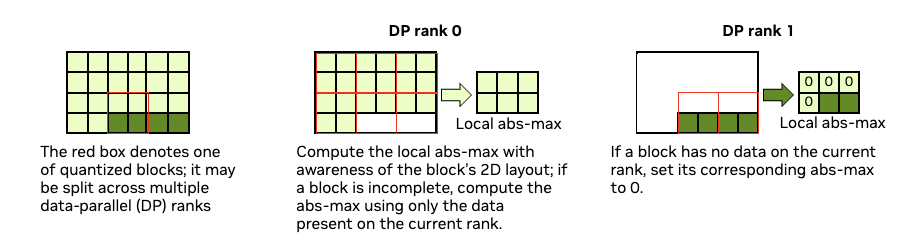
\includegraphics[width=1\linewidth]{figures/native_fp8_blockwise.png}
    \caption{用于按块缩放的 FP8 主要权重量化方案。}
    \label{fig:native_fp8_blockwise}
\end{figure}

\subsubsection{FP8/FP4 主要重量：消除冗余存储}\label{subsec:fp8-primary-weights}
传统的降低精度训练维持三层参数层次结构：用于优化器更新的 FP32 主权重、作为中间表示的 BF16 模型权重以及用于前向和后向 GEMM 计算的 FP8/FP4 权重。这通过维护 BF16 和 FP8/FP4 参数副本引入了冗余内存开销。

\textbf{本机 FP8/FP4} 通过建立从 FP32 主权重到 FP8/FP4 计算权重的直接转换路径，完全绕过 BF16 中间层，减少内存占用并加速参数 AllGather，消除了这种冗余。

实现原生 FP8/FP4 的核心挑战在于管理 FP8/FP4 张量所需的量化元数据。我们提供支持不同 FP8/FP4 配方（延迟缩放、电流缩放、块式缩放、MXFP8 和 NVFP4）的统一接口，处理 TransformerEngine 实现中特定于版本的差异，确保跨版本的兼容性。

在分布式优化器的每个优化器步骤中，FP32 参数分片都会根据减少的梯度进行更新。随后，这些更新的 FP32 分片使用适当的缩放因子直接量化为 FP8/FP4 格式。量化过程根据 FP32 值计算 amax，更新数据并行等级之间的缩放因子以保持一致性，并将量化的 FP8/FP4 值写入模型参数缓冲区。这种直接路径消除了维护 BF16 参数的内存开销，这对于参数内存可能超过数百 GB 的大型语言模型尤其有效。

更具体地说，延迟缩放和当前缩放的 FP32 分片的量化分三个步骤进行，请参阅 \figref{fig:native_fp8_current_scaling}:
\begin{itemize}
    \item 第 1 步：从主重量中获取局部最大腹肌。如果某个权重在当前rank上没有分片部分，则将其对应的abs-max设置为0。
    \item 步骤2：通过AllReduce获取全局abs-max。
    \item 第 3 步：使用全局最大腹肌和主权重进行部分投射。
\end{itemize}

\begin{figure}[ht]
    \centering
    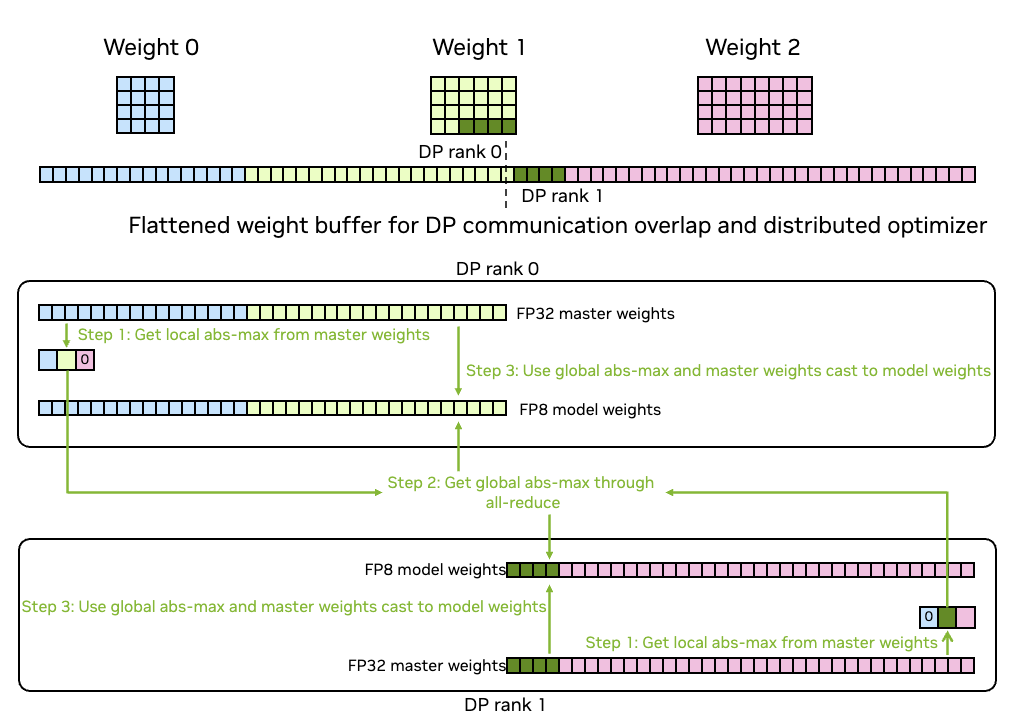
\includegraphics[width=1\linewidth]{figures/native_fp8_current_scaling.png}
    \caption{FP8 主要权重量化方案，用于延迟缩放和每张量当前缩放。}
    \label{fig:native_fp8_current_scaling}
\end{figure}

在Blockwise配方中，权重的abs-max是在2D块上计算的，因此我们不能直接使用归约内核来获得局部abs-max。我们实现了专门的内核，它了解权重的 2D 布局以及主权重和原始权重之间的对应关系，以计算ABS-MAX，请参阅 \figref{fig:native_fp8_blockwise}。

FP8/FP4初级权重的另一个优点是参数AllGather通信量大大减少（参见章节 \ref{sec:comm_wall_quantized_training}).


\subsection{教育部特有的低精度训练挑战和解决方案}

前面的小节介绍了适用于任何深度学习模型的降低精度训练的基础知识。 MoE 架构为降低精度的训练带来了独特的挑战，需要超出标准实施的专门解决方案。

\subsubsection{填充和取消填充的融合：动态形状对齐}
FP8 和 FP4 GEMM 要求张量维度与特定倍数对齐：每个张量和分块配方为 16，MXFP8 和 NVFP4 为 32。这些填充要求源自每个量化方案的块缩放粒度，以及张量内存加速器 (TMA) 访问沿 GEMM 点积维度保持 16 字节对齐的要求。在前向传递中，隐藏维度 K 是点积维度，通常已经通过模型设计进行了对齐。然而，在权重梯度GEMM中，点积维数对应于令牌维数M，其动态变化并且常常不能满足对齐要求。因此，沿着标记维度进行零填充是必要的。为了进一步启用具有较低 CPU 开销和 CUDA Graph 兼容性的分组量化内核，我们将每个专家的令牌填充增加到 128。 \ref{sec:fp4-quant-fusion} 解释了为什么 NVFP4 分组量化内核需要更大的填充；同样的原理也适用于 MXFP8 分组量化。总之，应用于令牌维度的最终填充是由路由专家层中涉及的所有内核的要求共同确定的。

我们的基线解决方案是针对不同专家的多个输入张量的融合填充和取消填充内核。然而，显式填充和取消填充内核会带来不可忽略的开销。我们提出两种解决方案：
\begin{itemize}
    \item \textbf{路由图填充}，它填充路由映射而不是接收到的令牌。这确保了每个专家的令牌数量符合要求，但代价是仅发送少量额外令牌，从而避免了昂贵的每个张量填充操作。
    \item \textbf{将填充融合到排列中} 避免全局内存读写的一次性传递，并应提供最佳性能。如果可用，它是默认选择。
\end{itemize}

% \subsubsection{FP8 EP Communications: Halving Dispatch Volume}\label{sec:fp8-dispatch-comm}
% With large EP strategies for fine-grained MoE models, EP communication becomes the primary bottleneck. To reduce this overhead, dispatch communication can be executed using FP8, halving the all-to-all volume.

% \textbf{Key insight}: Only the 1D per-token scaled recipe can make FP8 dispatch communication feasible (\figref{fig:fp8_dispatch}). In 1D per-token quantization, each token is associated with its own \textbf{row-wise} scaling factor tensor, which is preserved even after all-to-all communication. However, during weight gradient computation, the GEMM operation requires col-wise quantized (and optionally transposed) FP8 activations as input, which requires a dequantization and re-quantization (along another direction) step. To minimize potential accuracy loss due to double quantization, the E8M0 or power-of-two scale format is adopted.

% \begin{figure}[ht]
%     \centering
%     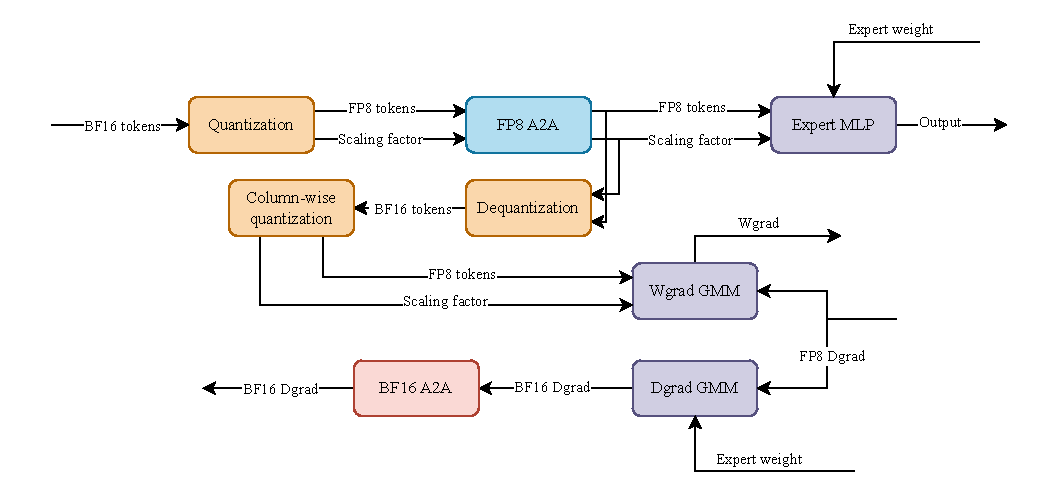
\includegraphics[width=1\linewidth]{figures/fp8_dispatch.drawio.pdf}
%     \caption{Using FP8 communication in the forward dispatch. The dequantization-quantization step is required for backward computation.}
%     \label{fig:fp8_dispatch}
% \end{figure}

% \paragraph*{Platform-Specific Implementations.}
% The blockwise recipe is used on Hopper, where FP8 GEMM only accepts inputs with a TN layout. This means the activation input must be row-major, so an additional transpose is required after column-wise quantization. In contrast, the MXFP8 recipe is employed on the Blackwell architecture, which supports arbitrary layouts and eliminates the need for this extra transpose.

% In the blockwise recipe, we need to quantize the tokens before communication. The quantized activations can directly participate in the forward computation. However, for the backward pass, we must first dequantize to reconstruct the high-precision input, then re-quantize to obtain the new result. This is because, for the same activation, the quantization dimensions used in the forward and backward phases are different. Since the Hopper Tensor Core only accepts specific layouts, a transposition step is also required beforehand.

% In the MXFP8 recipe, the process is almost identical to that of the blockwise method. Though transposition is unnecessary on the Blackwell platform, we still need the FP8 tensor quantized along different dimensions (col-wise vs. row-wise) for backward computation.

\subsubsection{分组量化和分组GEMM}

\paragraph{分组量化}

由于量化数据和缩放因子之间的填充要求不同，以及行量化和列量化引入的复杂数据布局，针对不同专家量化输入张量的一种简单方法是将量化内核逐个应用到它们。然而，它引入了大量的小内核，这增加了 CPU 开销，并且从 GPU 的角度来看效率不高。

为了解决这个问题，我们实现了分组量化内核，将多个张量的量化融合到一个内核中，这大大减少了 CPU 开销，提高了 GPU 利用率，并且是 CUDA-Graphable 的。

\paragraph{分组GEMM}
优化和 CUDA-Graphable 分组 GEMM 部分 \ref{sec:device-init}.


\subsubsection{NVFP4量化融合}\label{sec:fp4-quant-fusion}

由于我们使用数值技术来保持数值稳定性，NVFP4 量化尤其复杂，因此需要积极的内核融合来控制量化开销。在实践中，我们的 NVFP4 量化内核不仅仅是一个简单的“缩放 + 转换”内核：它需要仔细吸收训练配方逻辑，包括随机 Hadamard 变换、2D 缩放和随机舍入。 

其中，RHT 融合对延迟最敏感。如果作为单独的内核实现，Hadamard 变换将在全局内存中引入额外的全精度 (BF16) 张量读/写，从而显着增加带宽成本。通过将 RHT 与 NVFP4 量化融合，我们在单个内核中执行 Hadamard 变换和 FP4 量化，避免了额外的 BF16 流量。

第二个实施挑战是 Blackwell NVFP4 Tensor Core GEMM 是面向 TN 的，而 Wgrad 使用转置激活和梯度。因此，当 RHT 融合到 Wgrad 路径的 NVFP4 量化中时，内核还必须吸收转置，而不是依赖于单独的 BF16 转置内核（这将再次导致通过全局内存进行完整的 BF16 张量读写）。

因此，融合量化管道必须支持来自同一高精度输入的多个输出：(1) 前向 GEMM 的标准 FP4 量化，以及 (2) 后向/Wgrad 路径的转置 + RHT + FP4 量化。在训练中，我们在前向传递期间启动这个融合内核以生成两个 FP4 副本：一个由前向 GEMM 立即消耗，另一个保存用于后向。然后原始的高精度输入被丢弃，因此我们避免存储 BF16 激活，同时仍然有效地准备后向路径。

NVFP4 中的每个张量 FP32 尺度带来了进一步的复杂性。当前的 NVFP4 预训练方案，张量范围的 abs-max 是在 Hadamard 变换之后测量的，这意味着我们需要一个专用的 Hadamard+amax 内核来仅计算 amax（而不具体化变换后的 BF16 输出缓冲区）。因此，Hadamard 变换实际上被计算了两次——首先在 Hadamard-amax 内核中，然后在融合量化内核中再次计算。尽管这重复了变换计算，但它仍然比将完整变换的 BF16 张量写入全局内存更快的端到端速度，因为它避免了额外的高带宽 BF16 读/写流量。

相比之下，2D 量化在端到端吞吐量中不太明显，因为它仅适用于权重：我们可以对权重进行一次量化（例如，在第一个微批次上）并缓存量化的权重和比例，以便在以后的微批次中重用，因此其成本很大程度上被摊销。 

然而，随机舍入在关键路径上增加了内核级要求：量化内核还必须支持可选的随机舍入路径，并在内核中生成随机数（对于 dY 等梯度张量启用，否则禁用），以便 FP4 量化在单次传递中保持融合。为了保持效率，我们使用 NVIDIA cuRANDDx\cite{curanddx} 用于融合 CUDA 量化内核内的设备端随机数生成。

\paragraph{MoE 的分组 NVFP4 量化}

由于 NVFP4 配方本身的算法复杂性，支持 MoE 层的 NVFP4 量化尤其具有挑战性。在全迭代 CUDA Graph 要求下，MoE 量化路径也必须是 CUDA Graph 安全的：主机不能依赖于 CPU 上的动态专家令牌计数，而只能依赖于设备端每个专家令牌张量。这意味着输入激活不能再单独分割和量化。我们必须为完整的 NVFP4 管道实现分组量化内核。 NVFP4 输出的内存分配必须作为整个平面缓冲区进行分配，而不知道其间的形状。 

一个关键的观察结果是，大部分密集的 NVFP4 激活量化内核可以重新用于分组量化，因为不同专家的令牌在路由/排列后连续打包在内存中。主要区别在于保持性能和图形安全所需的实现限制。 

\begin{enumerate}

\item 量化线程块不应跨越多个专家的令牌，因为这会引入大量的控制流和索引开销；因此，我们将每个专家的令牌计数补零为令牌维度中线程块形状的整数倍（通常为 128）。 

\item NVFP4 转置必须针对每个专家执行（独立转置每个专家的打包激活，然后连接），这并不等同于将整个分组缓冲区转置为一个张量。 

\item NVFP4 GEMM 需要比例因子调配：比例因子必须填充为 128×4 对齐的形状，并在 GEMM 之前调配为 32×16 布局，如 cuBLAS 文档中所述\cite{cublas_sf_layout}。此缩放因子形状约束应用于每个专家 GEMM，这意味着确定所需的填充大小将隐式要求 CPU 对每个专家令牌的可见性，这不是 CUDA Graph 安全的。为了避免这种情况，我们通过构造强制每个专家 128 个令牌对齐。
\end{enumerate}

第 1) 点和第 3) 点都对每个专家施加了 128 个多个标记，这需要特定的零填充内核来满足。为了消除这种零填充开销，我们将每个专家的零填充功能融合到令牌排列内核中，因此路由的专家激活是在已经对齐和零填充的布局中生成的，并且下游分组的 NVFP4 量化/GEMM 内核可以假设所需的对齐，而无需额外的预处理。

对于 NVFP4 配方中的每张量 FP32 二级尺度，MoE 中的每张量二级尺度意味着每专家二级尺度，而不是让每个专家共享 amax 以在训练期间保持数值稳定性。这些 amax 值无法提前获知：它们必须根据路由令牌在线计算，并在每次迭代时生成为不同的每个专家 amax 值。为了有效地解决这个问题，我们利用每个专家 128 个对齐的令牌保证，并将密集输入实现调整为 CUDA-Graph 安全的分组 Hadamard-amax 内核。 

%==============================================================================
% SECTION 6: LONG-CONTEXT MOE TRAINING
%==============================================================================

